%---------------------------------------------------------------------
%	The MIT License (MIT)
%
%	Copyright (c) 2021 Jitin Nair
%
%	Permission is hereby granted, free of charge, to any person obtaining a copy
%	of this software and associated documentation files (the "Software"), to deal
%	in the Software without restriction, including without limitation the rights
%	to use, copy, modify, merge, publish, distribute, sublicense, and/or sell
%	copies of the Software, and to permit persons to whom the Software is
%	furnished to do so, subject to the following conditions:
%	
%	THE SOFTWARE IS PROVIDED "AS IS", WITHOUT WARRANTY OF ANY KIND, EXPRESS OR
%	IMPLIED, INCLUDING BUT NOT LIMITED TO THE WARRANTIES OF MERCHANTABILITY,
%	FITNESS FOR A PARTICULAR PURPOSE AND NONINFRINGEMENT. IN NO EVENT SHALL THE
%	AUTHORS OR COPYRIGHT HOLDERS BE LIABLE FOR ANY CLAIM, DAMAGES OR OTHER
%	LIABILITY, WHETHER IN AN ACTION OF CONTRACT, TORT OR OTHERWISE, ARISING FROM,
%	OUT OF OR IN CONNECTION WITH THE SOFTWARE OR THE USE OR OTHER DEALINGS IN
%	THE SOFTWARE.
%	
%---------------------------------------------------------------------

%---------------------------------------------------------------------
%	DOCUMENT DEFINITION
%---------------------------------------------------------------------

% article class because we want to fully customize the page and not use a cv template
\documentclass[a4paper,11pt]{article}

%---------------------------------------------------------------------
%	FONT
%---------------------------------------------------------------------

% % fontspec allows you to use TTF/OTF fonts directly
% \usepackage{fontspec}
% \defaultfontfeatures{Ligatures=TeX}

% % modified for ShareLaTeX use
% \setmainfont[
% SmallCapsFont = Fontin-SmallCaps.otf,
% BoldFont = Fontin-Bold.otf,
% ItalicFont = Fontin-Italic.otf
% ]
% {Fontin.otf}

%---------------------------------------------------------------------
%	PACKAGES
%---------------------------------------------------------------------
\usepackage{url}
\usepackage{parskip} 
%\usepackage[english]{babel}
\usepackage{csquotes}

%other packages for formatting
\RequirePackage{color}
\RequirePackage{graphicx}
\usepackage[dvipsnames]{xcolor}
\usepackage[left=1.5cm,top=1.cm,right=1.5cm,bottom=1.5cm,nofoot]{geometry}

%tabularx environment
\usepackage{tabularx}
\usepackage{booktabs}

%for lists within experience section
\usepackage{enumitem}

% centered version of 'X' col. type
\newcolumntype{C}{>{\centering\arraybackslash}X} 

%to prevent spillover of tabular into next pages
\usepackage{supertabular}
\usepackage{tabularx}
\newlength{\fullcollw}
\setlength{\fullcollw}{0.47\textwidth}

%custom \section
\usepackage{titlesec}				
\usepackage{multicol}
\usepackage{multirow}
\usepackage{tikz}
\usepackage{tikzpagenodes}
\usepackage{bm}
\usepackage{array, makecell}
\renewcommand\theadfont{\bfseries}
\usetikzlibrary{calc}
\usetikzlibrary{shapes.geometric}
\usetikzlibrary{decorations.pathmorphing}

%CV Sections inspired by: 
%http://stefano.italians.nl/archives/26
\titleformat{\section}{\Large\scshape\raggedright}{}{0em}{}[\titlerule]
\titlespacing{\section}{0pt}{10pt}{10pt}

%for publications
\usepackage[backend=biber, style=numeric, sorting=none]{biblatex}

%Setup hyperref package, and colours for links
\usepackage[unicode, draft=false]{hyperref}
\definecolor{linkcolour}{rgb}{0,0.2,0.6}
\hypersetup{colorlinks,breaklinks,urlcolor=linkcolour,linkcolor=linkcolour}
\addbibresource{citations.bib}
% Use the note field as the citation label and remove brackets
\DeclareFieldFormat{labelnumber}{\textbf{\thefield{note}}}
\renewcommand*{\labelalphaothers}{}

% Ensure numeric labels are cleared
\AtEveryBibitem{
  \clearfield{labelnumber}
}
%\setlength\bibitemsep{1em}

%for social icons
\usepackage{fontawesome5}
\usepackage{fancyhdr}

% remove word-splits
%\usepackage[none]{hyphenat}

% \newcommand\rating[2]{%
%   \pgfmathsetmacro\pgfxa{#1 + 1}%
%   \tikzstyle{scorestars}=[star, star points=5, star point ratio=2.25, draw, inner sep=0.15em, anchor=outer point 3]%
%   \begin{tikzpicture}[baseline]
%     \foreach \i in {1, ..., #2} {
%       \pgfmathparse{\i<=#1 ? "black" : "white"}
%       \edef\starcolor{\pgfmathresult}
%       \draw (\i*1.3em, 0) node[name=star\i, scorestars, fill=\starcolor]  {};
%     }
%     \pgfmathparse{#1>int(#1) ? int(#1+1) : 0}
%     \let\partstar=\pgfmathresult
%     \ifnum\partstar>0
%       \pgfmathsetmacro\starpart{#1-(int(#1))}
%       \path [clip] ($(star\partstar.outer point 3)!(star\partstar.outer point 2)!(star\partstar.outer point 4)$) rectangle 
%       ($(star\partstar.outer point 2 |- star\partstar.outer point 1)!\starpart!(star\partstar.outer point 1 -| star\partstar.outer point 5)$);
%       \fill (\partstar*1em, 0) node[scorestars, fill=yellow]  {};
%     \fi
%   \end{tikzpicture}%
% }

\newcommand{\skill}[3]{%
  \noindent
  \textsc{#1}
  \begin{minipage}[t]{0.15\linewidth}
    \begin{tikzpicture}[baseline={(0,0)}]
      \fill[gray!40, rounded corners=3pt] (0,0) rectangle (2,0.2);
      \fill[black!90, rounded corners=3pt] (0,0) rectangle (2*#2/#3,0.2);
    \end{tikzpicture}
  \end{minipage}%
}

%---------------------------------------------------------------------
%	BEGIN DOCUMENT
%---------------------------------------------------------------------
\begin{document}
% non-numbered pages
\pagestyle{fancy}
\fancyhf{} % sets both header and footer to nothing
\renewcommand{\headrulewidth}{0pt}
\setlength{\footskip}{4.08003pt}

%---------------------------------------------------------------------
%	TITLE
%---------------------------------------------------------------------
{\huge \textbf{Curriculum Vitae} \hfill \textit{Oscar Stommendal}} \\[-1cm]

\hrulefill

\vspace{-0.1cm}
{\small{}\textsc{BSc Engineering Physics $\vert$ MSc Physics $\vert$ BSc Business and Economics}}
\vspace{-0.1cm}

\begin{tabular}[l]{l|l|l|l|l|l}
    \small{}\hspace{-0.3cm} \href{mailto:oscar.stommendal01@gmail.com}{\raisebox{-0.05\height}\faEnvelope \ Email}& \small{}\href{tel:+46706617353}{\raisebox{-0.05\height}\faMobile \ iPhone} & \small{}\href{https://linkedin.com/in/oscar-stommendal} {\raisebox{-0.05\height}\faLinkedin\ LinkedIn} & \small{}\href{https://github.com/stommen} {\raisebox{-0.05\height}\faGithub \ Github} & \small{}\href{https://stommen.github.io}{\raisebox{-0.05\height}\faGlobe \ Personal Website} & \small{}\href{https://www.google.com/maps/place/Göteborg,+Sverige/@57.7005638,11.5642129,10z/data=!3m1!4b1!4m6!3m5!1s0x464f8e67966c073f:0x4019078290e7c40!8m2!3d57.70887!4d11.97456!16zL20vMDM0M18?entry=ttu&g_ep=EgoyMDI1MDEyOS4xIKXMDSoASAFQAw%3D%3D}{\raisebox{-0.05\height}\faMapMarker \ Gothenburg}
\end{tabular}
\hfill
% \begin{tikzpicture}[remember picture,overlay]
% \clip ($(current page text area.north east)!0.10!(current page text area.south east)!0.12!(current page text area.north west)$)
%   circle (2.2cm) node {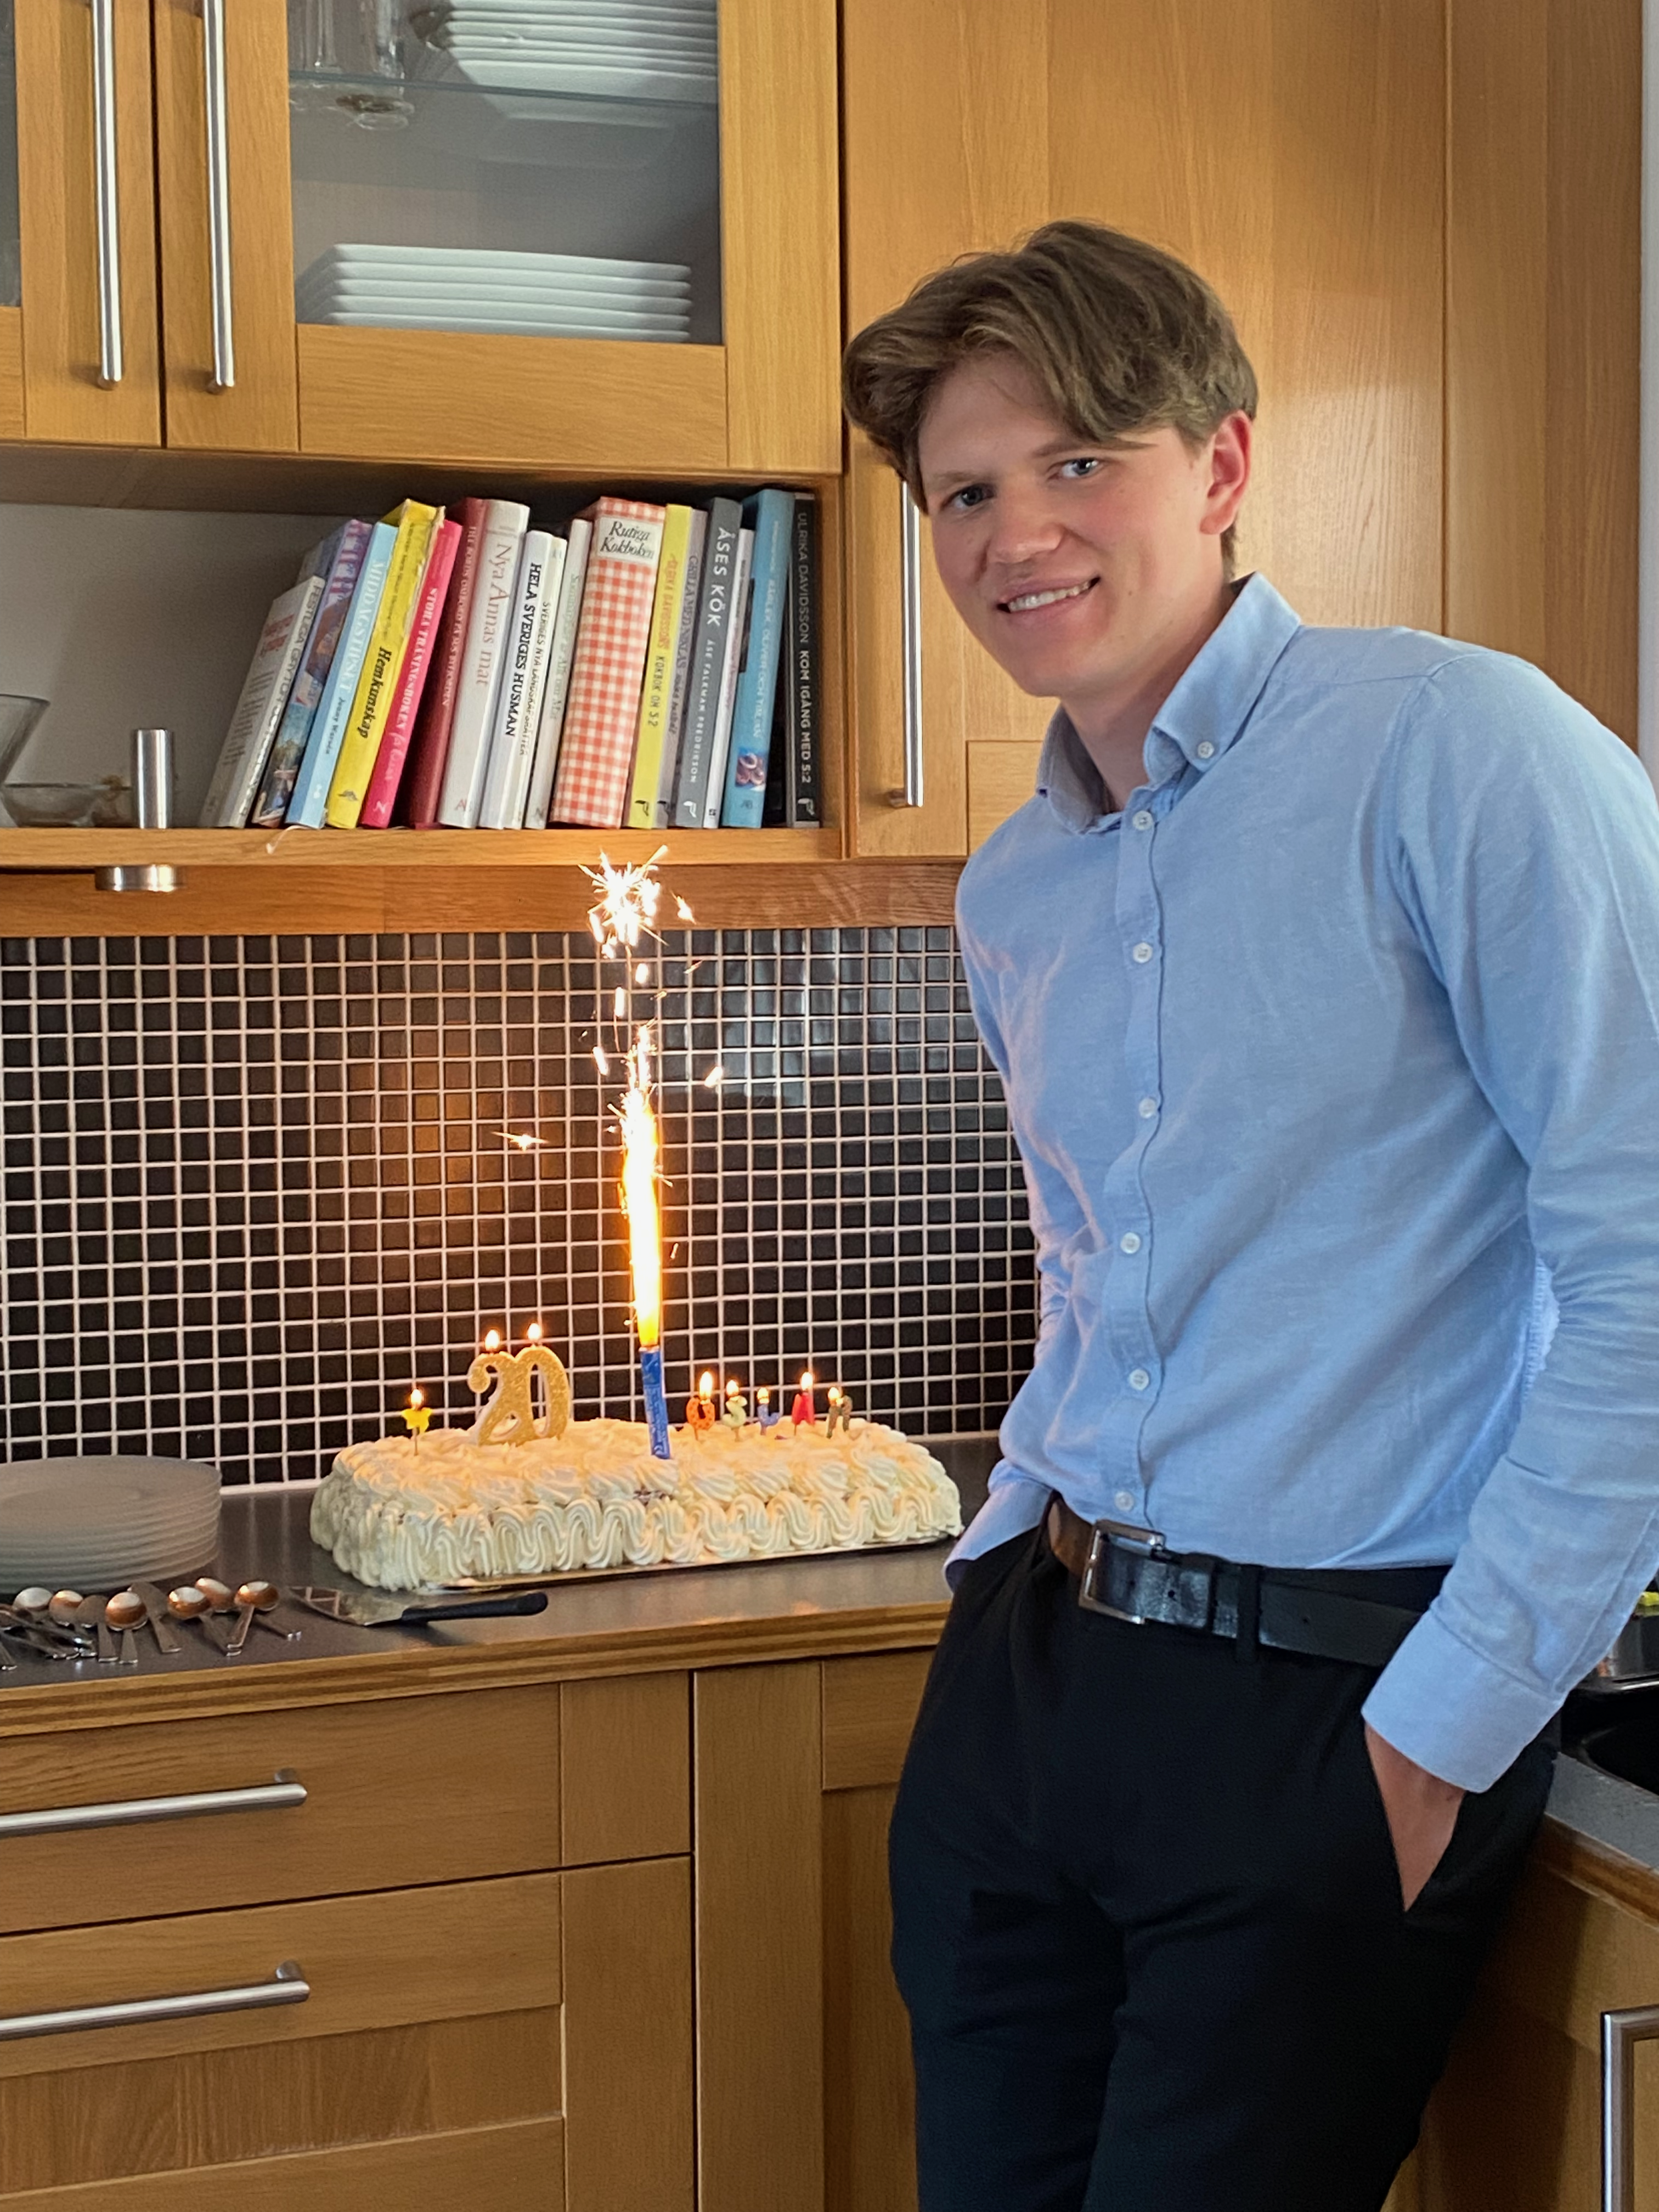
\includegraphics[width=4.5cm]{photos/cv_bild.pdf}};
% \end{tikzpicture}
\hspace*{0.1cm}\\[-0.6cm]

%---------------------------------------------------------------------
% Introduction
%---------------------------------------------------------------------
%Interests/ Keywords/ Summary
%\section{Goal with Application}
%By being a member of the NOVA talent network, I hope to gain valuable tips, insights and connections to help me kick-start my career. I hope to connect with like-minded peers and learn from experienced professionals who can guide me in my career path. 
%Through the CERN Summer Student Programme, I aim to deepen my understanding of science and technology while gaining experience in a world-class research environment. This opportunity will help me advance toward a future career at the forefront of technological advancements by collaborating with leading researcher and connecting with like-minded peers from around the world.
%Through a summer internship at Novatron, I hope to kick-start my career in the fusion- and renewable energy sector. I am eager to apply my knowledge in physics and engineering to real-world problems, and to learn from experienced professionals in the field. I am confident that my analytical skills, problem-solving abilities and positive attitude will make me a valuable addition to the team.
%At Ericsson, I hope to gain valuable experience and develop my engineering skills. I am eager to apply my knowledge in physics and engineering to real-world problems, and to learn from experienced professionals in the field. I am confident that my analytical skills, problem-solving abilities and positive attitude will make me a valuable addition to the team.
%At Nasdaq, I am very excited to apply my knowledge in physics, engineering and economics to solve real-world problems. I hope that the internship will provide me with valuable experience for a future career in the forefront of technological advancements at global-leading companies. I am confident that my skills and positive attitude will be a valuable addition to the team.
%At Spotify, I aim to merge my passion for music with my skills in physics, engineering, and economics to tackle real-world challenges. I am excited to learn from experienced professionals and gain valuable experience for a future career at globally leading companies, where I aspire to drive technological advancements and shape the future. With strong analytical skills, a problem-solving mindset, and a positive attitude, I am confident in my ability to contribute meaningfully to the team.
%At Amazon, I want to combine my skills in engineering and economics and tackle real-world challenges. I am excited to learn from experienced professionals and gain valuable experience for a future career at globally leading companies, where I aspire to drive technological advancements and shape the future. With strong analytical skills, a problem-solving mindset, and a positive attitude, I am confident in my ability to contribute meaningfully to the team.
%Through a summer internship at Volvo, I hope to gain valuable experience by applying my knowledge in physics and engineering to real-world problems. I am excited to learn from professionals and gain valuable experience for a future career at globally leading companies, where I aspire to drive technological advancements and shape the future. With strong analytical skills, a problem-solving mindset, and a positive attitude, I am confident in my ability to contribute meaningfully to the team.%I see this as a golden opportunity to grow professionally by adding experience in CFD and aerodynamics to my toolbox, since I have not yet had the opportunity to work with these areas. As a quick learner, together with my analytical skills and problem-solving abilities, I am confident that I can contribute to the team.
%At Zenseact, I hope to gain valuable experience and develop my engineering skills. I am eager to apply my knowledge in physics and engineering to real-world problems, and to learn from experienced professionals in the field. I am confident that my analytical skills, problem-solving abilities and positive attitude will make me a valuable addition to the team.
%As a large sports car enthusiast, I am very excited about the opportunity to work at Koenigsegg. I hope to gain valuable experience and develop my engineering skills for a future career in the forefront of technology, where I can shape the future of the automotive industry. I am eager to apply my knowledge in physics and engineering to real-world problems, and to learn from experienced professionals in the field. With my analytical skills, problem-solving abilities and positive attitude, I am confident that I can contribute to the team.
%At Beyond Gravity, I aim to merge my passion for space with my skills in physics, programming and engineering to tackle real-world challenges. I am excited to learn from experienced professionals and gain valuable experience for a career at the forefront of technology, where I aspire to drive and shape the future. With strong analytical and programming skills, a problem-solving mindset, and a positive attitude, I am confident in my ability to contribute meaningfully to the team.
%At Coherent, I hope to gain valuable experience and develop my engineering skills. I am eager to apply my knowledge in physics and engineering to real-world problems, and to learn from experienced professionals in the field. I am confident that my analytical skills, problem-solving abilities and positive attitude will make me a valuable addition to the team.
%At Hitachi, I aim to merge my passion for a green future with my skills in physics and engineering to tackle real-world challenges. I am excited to learn from experienced professionals and gain valuable experience for a future career at globally leading companies, where I aspire to drive technological advancements and shape the future. With strong analytical skills, a problem-solving mindset, and a positive attitude, I am confident in my ability to contribute meaningfully to the team.
%At Saab, I hope to gain valuable experience and develop my engineering skills. I am eager to apply my knowledge in physics and engineering to real-world problems, and to learn from experienced professionals in the field. I am confident that my analytical skills, problem-solving abilities and positive attitude will make me a valuable addition to the team.
%Working in car climate at Volvo, I hope to gain valuable experience and develop my engineering skills. I am eager to apply my knowledge in physics and engineering to real-world problems, and to learn from experienced professionals in the field. I am confident that my analytical and programming skills, problem-solving abilities and positive attitude will make me a valuable addition to the team.
%At Zeekr, I hope to gain valuable experience and develop my engineering skills. I am eager to apply my knowledge in physics and engineering to real-world problems, and to learn from experienced professionals in the field. I am confident that my analytical skills, problem-solving abilities and positive attitude will make me a valuable addition to the team.
%Working with Bosonic Quantum Computation at Chalmers, I hope to apply my theoretical knowledge in quantum mechanics and computing to cutting-edge research. I am eager to work with experienced professionals and gain valuable experience for a future career at the forefront of technology, hopefully within quantum computing. The latter I also hope to achieve by broaden my network and make new connections within the field of quantum computing. 
%Working with Superconducting Circuit Platforms in WACQT at Chalmers, I hope to apply my theoretical knowledge in quantum mechanics and computing to cutting-edge research. I am eager to work with experienced professionals and gain valuable experience for a future career at the forefront of technology, hopefully within quantum computing. The latter I also hope to achieve by broaden my network and make new connections within the field of quantum computing. 
%At Ericsson, I hope to apply my theoretical knowledge in quantum mechanics and computing to real-world problems. I am eager to work with professionals and gain valuable experience for a future career at the forefront of technology, hopefully within quantum computing. The latter I also hope to achieve by broadening my network within the field of quantum computing and developing my engineering skills further.
%By an internship at the Feynman Quantum Academy, I hope to deepen my understanding of quantum and quantum -computing while gaining practical experience in a motivating environment, where I can learn from experienced professionals and collaborate with like-minded peers.
%Motivated by Bain's commitment to result-driven strategies, collaborative culture, and forward-thinking work in sustainability, finance and tech, I seek an associate internship to contribute with my unique mix of physics and economics. I'm eager to solve complex problems in an encouraging, dynamic and challenging environment while learning from world-class teams that challenge and inspire me to grow into a leader who can shape the future.
%I'm eager to learn from skilled professionals and gain valuable experience for a future career at the forefront of technology, where I aspire to shape the future. I'm especially interested in Bain's work in sustainability, financial services and technology.
%Motivated by a deep curiosity for fundamental physics, I seek a CERN studentship to contribute to cutting-edge research while gaining practical experience in an encouraging, world-class environment. I'm eager to learn from experts and collaborate on meaningful projects — which will help me pursue a future career at the forefront of technological innovation. I'm particularly interested in CERN's work on cosmology, quantum computing and fusion energy.
% \section{Motivation and Relevant Skills}
% \begin{itemize}[itemsep=1pt]
    % \item[$\bm{\star}$] Practical experience within engineering and collaborative problem-solving through internships
    %\item[\footnotesize{\textbf{\faCheckCircle}}] Unique combination of complex problem-solving, leadership and strategic thinking skills
    %\item[$\bm{\star}$] Coursework in nuclear physics, computational physics, plasma physics and quantum computing%, open quantum systems and quantum optimization
    %\item[$\bm{\star}$] (Collaborative) Programming: Python, Microsoft Office, Matlab, C and Git
    %\item[$\bm{\star}$] Collaborative laboratory work and report writing
    %\item[$\bm{\star}$] Hands-on experience in advanced experimental physics and data analysis, with projects in quantum physics, nuclear physics, solid-state physics, optics, and thermodynamics
    %\item[$\bm{\star}$] Collaborative laboratory work and programming: Python, Matlab, C, C++ and Git
    %\item[$\bm{\star}$] Positive team player with good communication skills and a passion for problem-solving
    %\item[$\bm{\star}$] Highly competitive, analytical, curious, detail-oriented, fast learner and methodical
    % \item[$\bm{\star}$] Goal-oriented and competitive -- hence very result-oriented
    % \item[\footnotesize{\textbf{\faCheckCircle}}] Former exchange student at NTU Singapore who enjoys working with others and meeting new people
    % \item[\footnotesize{\textbf{\faCheckCircle}}] Ambition to inspire other Chalmers students to go abroad, as I had the adventure of a lifetime
%\end{itemize}

%---------------------------------------------------------------------
%	EDUCATION
%---------------------------------------------------------------------
\section{Education}
\begin{tabularx}{\linewidth}{@{}l X@{}}	
2024 - now &MSc Physics at \textbf{Chalmers University of Technology} \hfill GPA: 5.0/5.0\\
&\textit{Focus on computational physics, astronomy and quantum physics/computing.} \\[5pt]

2025 &Exchange Semester at \textbf{Nanyang Technological University}, Singapore \\
&\textit{QS World University Ranking 12. Advanced topics in physics, business, and engineering.} \\[5pt]

2023 - now &BSc Business and Economics at \textbf{University of Gothenburg} \hfill \\[5pt] 

2020 - 2023 &BSc Engineering Physics at \textbf{Chalmers University of Technology} \hfill GPA: 4.3/5.0\\
&Bachelor's Thesis: \textit{Gibbs objective function for modification of the optimization process in a hybrid quantum algorithm} \\[18pt]

2017 - 2020 &Natural Sciences program at \textbf{Nils Ericson High School} \hfill GPA: 4.8/5.0
\end{tabularx}

%---------------------------------------------------------------------
%Experience
%---------------------------------------------------------------------
\section{\texorpdfstring
  {Work Experience \hfill \footnotesize\textsuperscript{\textcolor{black}{\faInfoCircle}} \textit{References available.}}
  {Work Experience (References available.)}}
\begin{tabularx}{\linewidth}{ @{}l r@{} }
\textbf{Summer Internship within Emerging Compute @ \textit{Ericsson}}\textsuperscript{\textcolor{black}{\faInfoCircle}} & \hfill Jun 2025 - now \\[3.75pt]
\multicolumn{2}{@{}X@{}}{
\begin{minipage}[t]{\linewidth}
    \begin{itemize}
        \item[--] Investigated the potential of quantum computing to solve problems in telecommunications.
        \item[--] Contributed to cutting-edge research, R\&D strategy discussions, and worked in cross-functional teams.
    \end{itemize}
\end{minipage}}
\end{tabularx}

\begin{tabularx}{\linewidth}{ @{}l r@{} }
\textbf{Research Technician @ \textit{GKN Aerospace}}\textsuperscript{\textcolor{black}{\faInfoCircle}} & \hfill Sep 2023 - May 2024 \\[3.75pt]
\multicolumn{2}{@{}X@{}}{
\begin{minipage}[t]{\linewidth}
    \begin{itemize}
        \item[--] Optimized MATLAB and Python tools, cutting processing time and speeding engineering decisions.
        \item[--] Developed a Python package to automate QA, cutting preparation time and improving consistency.
        \item[--] Coordinated with engineers and project managers to align tool improvements with operational needs.
    \end{itemize}
\end{minipage}}
\end{tabularx}

\begin{tabularx}{\linewidth}{ @{}l r@{} }
\textbf{Summer Internship in the GTC-department @ \textit{GKN Aerospace}}\textsuperscript{\textcolor{black}{\faInfoCircle}} & \hfill Jun 2023 - Aug 2023 \\[3.75pt]
\multicolumn{2}{@{}X@{}}{
\begin{minipage}[t]{\linewidth}
    \begin{itemize}
        \item[--] Automated data analysis and developed a tool for stress calculations on CAD models using Python.
        \item[--] Reduced the time spent on data analysis, improving the department's overall efficiency.
    \end{itemize}
\end{minipage}}
\end{tabularx}

\begin{tabularx}{\linewidth}{ @{}l r@{} }
    \textbf{Part-time Consultant @ \textit{Nordisk rörmärkning AB}}\textsuperscript{\textcolor{black}{\faInfoCircle}} & \hfill Apr 2021 - Nov 2023 \\[3.75pt]
    \multicolumn{2}{@{}X@{}}{
    \begin{minipage}[t]{\linewidth}
        \begin{itemize}
            \item[--] Designed Excel/VBA tools to automate and simplify customer orders, minimizing efforts and errors.
        \end{itemize}
    \end{minipage}
    }
\end{tabularx}

% \begin{tabularx}{\linewidth}{ @{}l r@{} }
% \textbf{Cashier summer work @ \textit{ICA Supermarket Mellerud}}\textsuperscript{\textcolor{black}{\faInfoCircle}} & \hfill Jun 2020 - Aug 2022 \\[3.75pt]
% \multicolumn{2}{@{}X@{}}{
%   \begin{minipage}[t]{\linewidth}
%     \begin{itemize}
%       \item[--] Mentoring new-starters and general people skills development.
%     \end{itemize}
%   \end{minipage}
% }
% \end{tabularx}

%\begin{tabularx}{\linewidth}{ @{}l r@{} }
% \textbf{Summer work @ \textit{Norra Älvsborgs Länssjukhus (NÄL)}} & \hfill Jul 2019 - Aug 2019 \\[5pt]
% \multicolumn{2}{@{}X@{}}{Kitchen responsibility at the X-ray department. I also got to see a lot of the work on the department.} \\[10.75pt]
%\end{tabularx}

%---------------------------------------------------------------------
%	SKILLS
%---------------------------------------------------------------------
\section{Qualifications}
\begin{minipage}[t]{0.82\textwidth}
  \textbf{\underline{Programming and Software Knowledge}} \\[10pt]
  %\raggedright
  %\renewcommand{\arraystretch}{1.25}
  %\setlength{\tabcolsep}{15pt}
  %\vspace*{-\topskip}
  % \centering
  % \begin{tabular}{lll}
  %   %\toprule
  %   \makecell{\thead{Highly Proficient} \\
  %   \rating{5}{5}} & \makecell{\thead{Proficient} \\ \rating{3}{5}} & \makecell{\thead{Basic} \\ \rating{1}{5}} \\ \toprule
  %   \makecell{Python \\ Matlab \\ Microsoft Office \\ GitHub \\ Git} & \makecell{C++ \\  C \\ \LaTeX \\ Linux \\ Azure} & \makecell{HTML \\ YAML \\ ANSYS \\ Visual Basic \\ LabVIEW} \\[10pt] \bottomrule
  % \end{tabular}
  \skill{}{5}{5}Highly Proficient: Python, MATLAB, Microsoft Office, Git/GitHub \\[5pt]
  \skill{}{3}{5}Proficient: C/C++, \LaTeX, Linux, Azure \\[5pt]
  \skill{}{1}{5}Basic: HTML, YAML, ANSYS, Visual Basic, LabVIEW
\end{minipage}
\begin{minipage}[t]{0.18\textwidth}
  \textbf{\underline{Languages}} \\[10pt]
  Swedish (Native) \\[5pt]
  English (C2) \\[5pt]
  Spanish (A1)
\end{minipage}

\section{Extracurricular Activities}
\begin{tabularx}{\linewidth}{ @{}l X@{}}
2022 & Qualified for \textbf{Mensa Sweden} \\[5pt]
2020 & \textbf{Intize mentor} for high-school students in math and physics \\[5pt]
2009 - 2018 & \textbf{Floorball player}, including 3 seasons as captain/leader of the team
\end{tabularx}
\section{Additional Information}
\textbf{\underline{Scholarships:}} Anna Whitlocks Minnesfond, Doktor Felix Neuberghs Stiftelse, Stiftelsen AAA. \\[8pt]
\textbf{\underline{Interests}:} Personal projects in finance and programming, music, food, skiing, sports, fitness, traveling.

\end{document}
